\data{14/11/2019}
\chapter{Support Vector Machine}
%TODO $\varepsilon$ and $\epsilon$ are swapped\newline
Support Vector Machines (SVM) are linear classifiers selecting a hyperplane such that the separation maximize the separation margin between classes. They are also called \textbf{large margin} classifiers.\newline
The solution actually depends only on a small subset of training examples, called \textbf{support vectors}. \newline
It also present a sound generalization theory and it can be easily extended to nonlinear separation with \textit{kernel machines}.
%
%
%
\section{Maximum Margin Classifier}
Given a training set $\mathcal{D}$, a classifier \textit{confidence} margin is the minimal confidence margin (for predicting a true label) among training examples:
\[\rho=\min\limits_{(\vect{x},y)\in\mathcal{D}}yf(\vect{x})\]
Instead a classifier \textit{geometric margin} is:
\[\frac{\rho}{\vert\vert\vect{w}\vert\vert}=\min\limits_{(\vect{x},y)\in\mathcal{D}}\frac{yf(\vect{x})}{\vert\vert\vect{x}\vert\vert}\]
There is an infinite number of equivalent formulation for the same hyperplane. Indeed if the following is true:
\[\vect{w}^T\vect{x}+w_0=0\]
then:
\[\alpha(\vect{w}^T\vect{x}+w_0)=0\quad\forall\alpha\neq 0\]
The \textbf{canonical hyperplane} is the one having confidence margin equal to 1:
\[\rho=\min\limits_{(\vect{x},y)\in\mathcal{D}}yf(\vect{x})=1\]
and its geometric margin is:
\[\frac{\rho}{\vert\vert\vect{w}\vert\vert}=\frac{1}{\vert\vert\vect{w}\vert\vert}\]
\begin{center}
  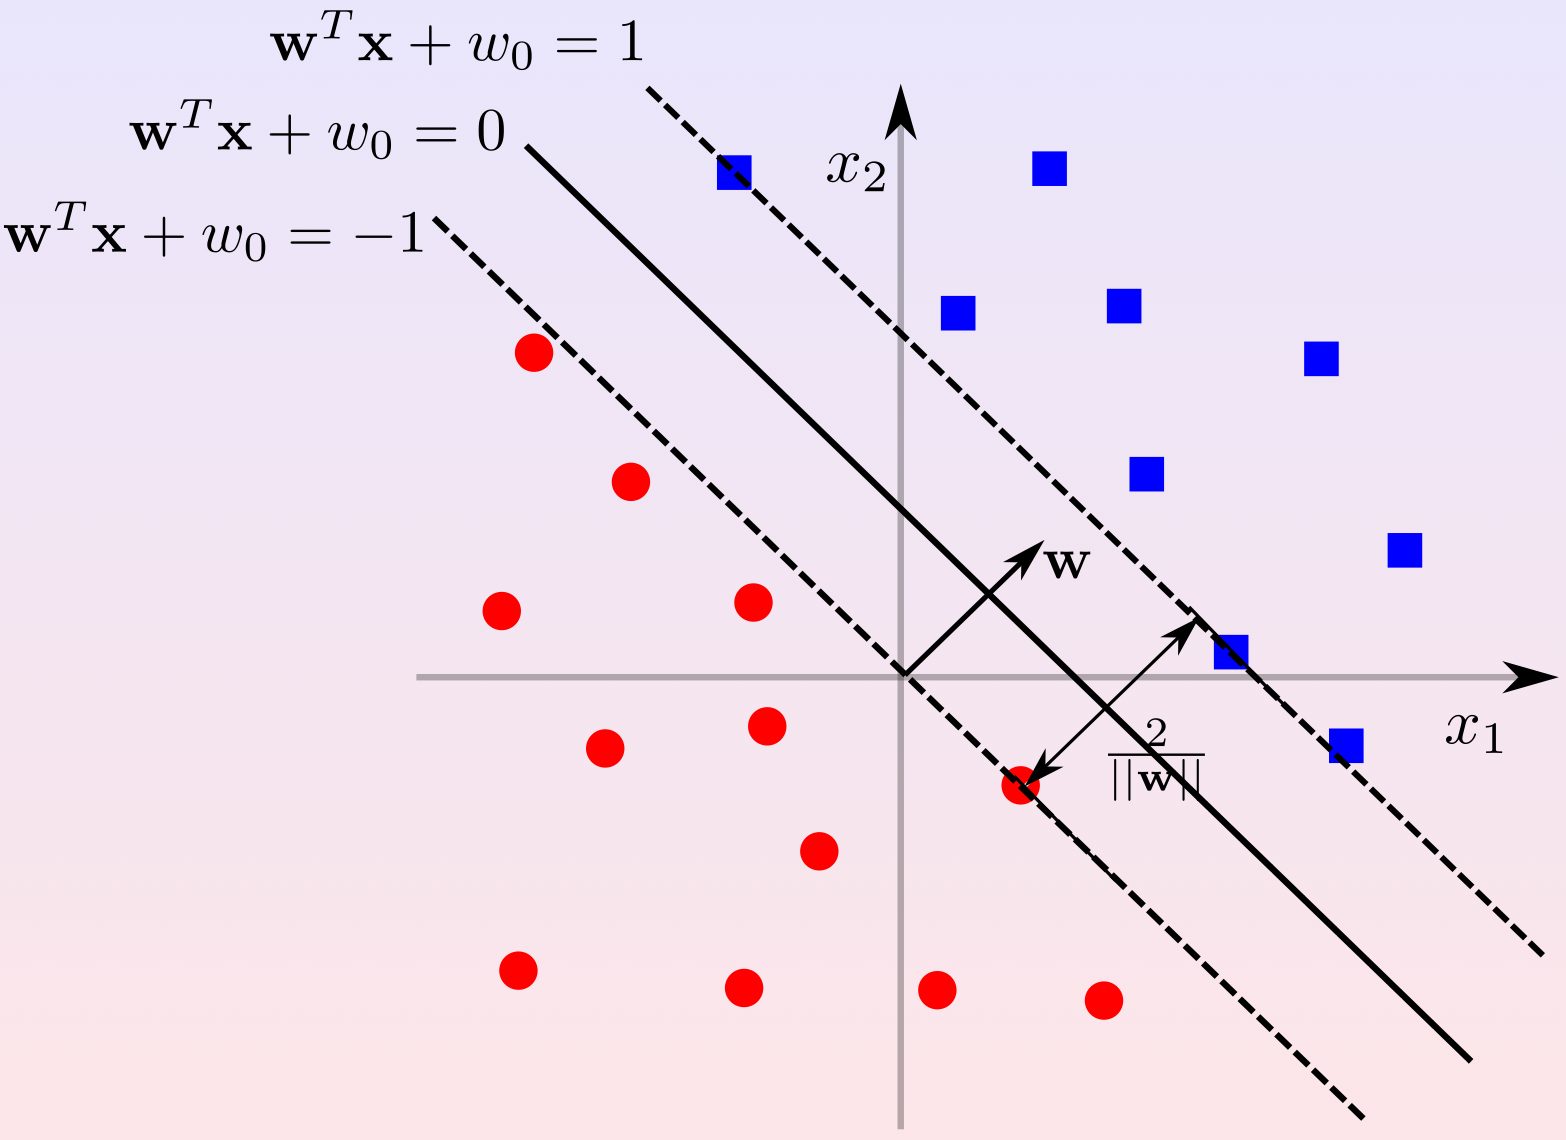
\includegraphics[width=0.7\linewidth]{SVM1}
\end{center}
%
%
%
\section{Hard Margin SVM}
\begin{theorem}[Margin Error Bound]
  Consider the set of decision functions $f(\vect{x})=\sign{\vect{w}^T\vect{x}}$ with $\vert\vert\vect{w}\vert\vert\leq \wedge$ and $\vert\vert\vect{x}\vert\vert\leq R$, for some $R,\wedge>0$. Moreover, let $\rho>0$ and $v$ denote the fraction of training examples with margin smaller than $myfrac{\rho}{\vert\vert\vect{w}\vert\vert}$, referred to as the \textbf{margin error}. \newline
  For all distributions $P$ generating the data, with probability at least $1-\delta$ over the drawing of the $m$ training patterns, and for any $\rho>0$ and $\delta\in(0,1)$, the probability that a test pattern drawn from $P$ will be misclassified is bound from above by:
  \begin{equation}
    v+\sqrt{\frac{c}{m}\left(\frac{R^2\wedge^2}{\rho^2}\ln^2m+\ln\left(\frac{1}{\delta}\right)\right)}
    \label{eq:MarginErrorBound}
  \end{equation}
  where $c$ is a universal constant.
\end{theorem}
What the theorem says is that the probability of test error depends on (among other components):
\begin{itemize}
  \item The number of margin errors $v$, that is examples with margin smaller than $\myfrac{\rho}{\vert\vert\vect{w}\vert\vert}$;
  \item The number of training examples, indeed the error depends on $\myfrac{\ln^2m}{m}$;
  \item The size of the margin, the error depends on $\myfrac{1}{\rho^2}$.
\end{itemize}
Notice that if we are considering the canonical hyperplane, then $\rho=1$ and the problem corresponds to minimizing $\vert\vert\vect{w}\vert\vert$:
\[
  \min\limits_{\vect{w},w_0}\frac{1}{2}\vert\vert\vect{w}\vert\vert^2\quad\text{subject to:}\quad y_i(\vect{w}^T\vect{x}_i+w_0)\geq 1\quad\forall (\vect{x}_i,y_i)\in\mathcal{D}
\]
The constraint guarantees that all points are correctly classified. \newline
Notice that this minimization corresponds to maximizing the (squared) margin. 
%
%
\subsection{Karush-Kuhn-Tucker Approach (KKT)}
This approach starts from the fact that a constrained optimization problem can be addressed by converting it into an unconstrained problem with the same solution. \newline
Let's have a constrained optimization problem in the form:
\[\min\limits_zf(z)\quad\text{subject to:}\quad g_i(z)\geq 0\forall i\]
Now we can introduce a non-negative variable $\alpha_i\geq0$, called Langrange multiplier, for each constraint and rewrite the optimization problem in the form of a Langrangian:
\[\min\limits_z\max\limits_{\alpha\geq0}f(z)-\Sum_i\alpha_ig_i(z)\]
The optimal solutions $z^*$ for this problem are the same as the optimal solutions for the original (constrained) problem:
\begin{itemize}
  \item If for a given $z'$ at least one constraint is not satisfied, i.e., $g_i(z')<0$ for some $i$, then maximizing over $\alpha_i$ leads to an infinite value;
  \item If all constraints are satisfied, i.e., $g_i(z')\geq0\forall i$, then the maximization over the $\vect{\alpha}$ will set all elements of the summation to zero, so that $z'$ is a solution of $\min\limits_zf(z)$.
\end{itemize}
The KKT approach can be used to solve the hard margin SVM constraint by rewriting the problem with a Langrangian as: 
\[\mathcal{L}(\vect{w},w_0,\vect{\alpha})=\frac{1}{2}\vert\vert\vect{w}\vert\vert^2-\Sum_{i=1}^m\alpha_i\left(y_i(\vect{w}^T\vect{x}_i+w_0)-1\right)\]
where $m=\vert\mathcal{D}\vert$.
The Langrangian is minimized w.r.t. $\vect{w}, w_0$, called the \textbf{primal variables} since they were in the original problem, and maximized w.r.t. $\alpha_i$, called \textbf{dual variables}. The solution is a saddle point. When the Langrangian is minimized and then maximized, we obtain a \textbf{dual formulation} since the only variables that will remain are the dual variables. \newline
Let's then first minimize over $\vect{w}$ and $w_0$:
\[\frac{\partial}{\partial\vect{w}}\mathcal{L}(\vect{w},w_0,\vect{\alpha})=0\]
\[\frac{\partial}{\partial\vect{w}}\left(\frac{1}{2}\vert\vert\vect{w}\vert\vert^2-\Sum_{i=1}^m\alpha_i\left(y_i(\vect{w}^T\vect{x}_i+w_0)-1\right)\right)=\vect{w}-\Sum_{i=1}^m\alpha_iy_i\vect{x}_i=0\]
\begin{equation}
  \vect{w}=\Sum_{i=1}^m\alpha_iy_i\vect{x}_i
  \label{eq:PrimalVariablew}
\end{equation}
\[\frac{\partial}{\partial w_0}\mathcal{L}(\vect{w},w_0,\vect{\alpha})=0\]
\[\frac{\partial}{\partial w_0}\left(\frac{1}{2}\vert\vert\vect{w}\vert\vert^2-\Sum_{i=1}^m\alpha_i\left(y_i(\vect{w}^T\vect{x}_i+w_0)-1\right)\right)=-\Sum_{i=1}^m\alpha_iy_iw_0=0\]
\[\Sum_{i=1}^m\alpha_iy_iw_0=0\]
We can now substitute in the Langrangian and then maximize for $\vect{\alpha}$:
\[\frac{1}{2}\vert\vert\vect{w}\vert\vert^2-\Sum_{i=1}^m\alpha_i\left(y_i(\vect{w}^T\vect{x}_i+w_0)-1\right)=\]
\[=\frac{1}{2}\left(\Sum_{i=1}^m\alpha_i\vect{x}_iy_i\right)^T\left(\Sum_{j=1}^m \alpha_j\vect{x}_jy_j\right)-\Sum_{j=1}^m\vect{x}_j\alpha_j\left(\Sum_{i=1}^m\vect{x}_iy_i\alpha_i\right)^T\vect{x}_j-\Sum_{i=1}^my_i\alpha_iw_0+\Sum_{i=1}^m \alpha_i\]
Since only $\vect{x}$ is a vector, we can take all the rest out of the transpose:
\[\frac{1}{2}\Sum_i\Sum_j\alpha_i\alpha_jy_iy_j\vect{x}_i^T\vect{x}_j-\Sum_i\Sum_j\alpha_i\alpha_jy_iy_j\vect{x}_j^T\vect{x}_i+\Sum_i\alpha_i\]
\[=\Sum_i\alpha_i-\frac{1}{2}\Sum_i\Sum_j\alpha_i\alpha_jy_iy_j\vect{x}_i^T\vect{x}_j\]
It's possible to notice that this actually is a Langrangian over the dual variables $\vect{\alpha}$ obtaining the \textit{dual formulation}:
\begin{equation}
  \mathcal{L}(\vect{\alpha})=\Sum_i\alpha_i-\frac{1}{2}\Sum_i\Sum_j\alpha_i\alpha_jy_iy_j\vect{x}_i^T\vect{x}_j
  \label{eq:DualFormulation}
\end{equation}
We now have to maximize over all possible $\vect{\alpha}$:
\[
  \max\limits_{\vect{\alpha}\in\mathbb{R}^m}\Sum_{i=1}^m\alpha_i-\frac{1}{2}\Sum_{i,j=1}^m\alpha_i\alpha_jy_iy_j\vect{x}_i^T\vect{x}_j\quad\text{subject to:}\quad 
\begin{cases}
  \alpha_i\geq0,\quad i=1,\hdots, m\\
  \Sum_{i=1}^m\alpha_iy_i=0
\end{cases}
\]
Mind that this is still a quadratic problem with linear constraints. The advantage with the dual formulation is the fact that the constraints are much simpler: non-negativity and "box"-constraint VS the original problem constraints, which were an hyperplanes. \newline
Notice that the primal formulation has $d+1$ variables, that is the number of features plus one:
\[\min\limits_{\vect{w},w_0}\frac{1}{2}\vert\vert\vect{w}\vert\vert^2\]
The dual formulation has $m$ variables, that is the number of training examples:
\[\max\limits_{\vect{\alpha}\in\mathbb{R}^m}\Sum_{i=1}^m\alpha_i-\frac{1}{2}\Sum_{i,j=1}^m\alpha_i\alpha_jy_iy_j\vect{x}_i^T\vect{x}_j\]
So one could choose the primal formulation if it has much less variables. \newline
We can then substitute Equation~\ref{eq:PrimalVariablew} into the decision function and obtain:
\[f(\vect{x})=\vect{w}^T\vect{x}+w_0=\Sum_{i=1}^m\alpha_iy_i\vect{x}_i^T\vect{x}+w_0\]
This tells us how the decision function works on the samples: we are predicting $\vect{x}$ with the bias $w_0$ and then multiply each example $\vect{x}_i$ by $\vect{x}$ with the dot product. The result of the dot product is higher if the two vectors are aligned, so we are basically trying to find a similarity. Then each result is combined with a weight $\alpha_i$ so that if the weight is actually large, $y_i$ is more probable to be the correct outcome. \newline
\data{14-11-2019}
At the saddle point it holds that:
\[\alpha_i\left(y_i\left(\vect{w}^T\vect{x}_i+w_0\right)-1\right)=0,~ \forall i\]
For this to be true, either:
\begin{itemize}
  \item the example does not contribute to the final $f(\vect{x})$, hence $\alpha_i=0$,
  \item or the example stays on the minimal confidence hyperplane from the decision:
    \[y_i\left(\vect{w}^T\vect{x}_i+w_0\right)=1\]
\end{itemize}
\begin{center}
  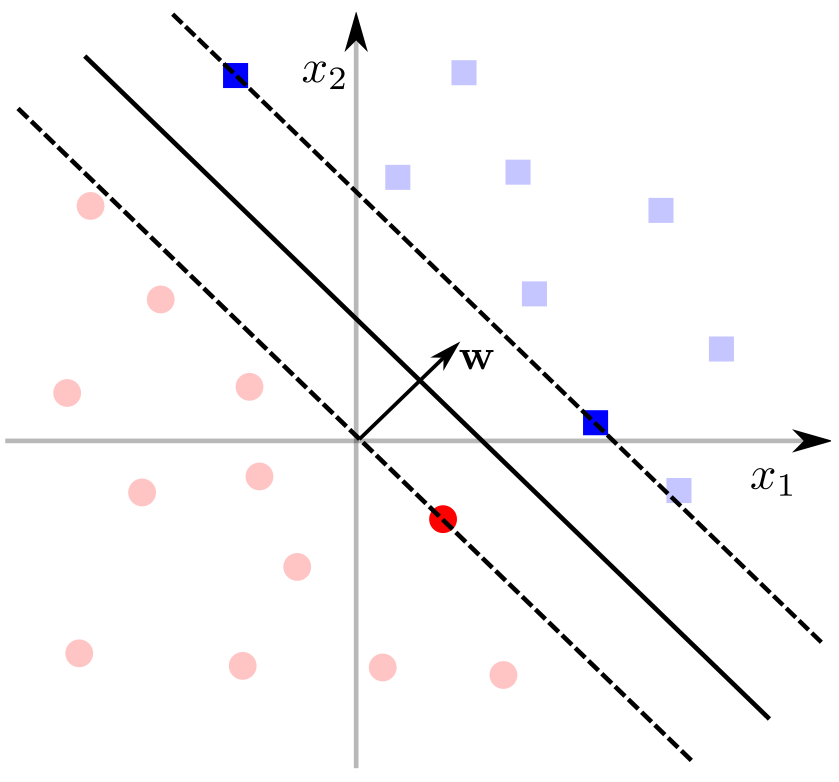
\includegraphics[width=0.7\linewidth]{HardMarginSVM}
\end{center}
All the points staying on the minimal confidence hyperplanes are called \textbf{support vectors} and are such that $\alpha_i\neq 0 \wedge y_i\left(\vect{w}^T\vect{x}_i+w_0\right)=1$. These are the only points that contribute to the final decision function, all the others do not matter, i.e., they could be even removed from the training set. 
SVMs are often \textit{sparse} since it is made of very few examples. \newline
The bias $w_0$ can be computed from the KKT conditions: given an arbitrary support vector $\vect{x}_i$ with $\alpha_i>0$, the KKT conditions imply:
\[y_i\left(\vect{w}^T\vect{x}_i+w_0\right)=1\]
\[y_i\vect{w}^T\vect{x}_i+y_iw_0=1\]
\[w_0=\frac{1-y_i\vect{w}^T\vect{x}_i}{y_i}\]
For robustness, the bias is usually averages over all support vectors. \newline
All this though leads to a possible problem. Let's consider the following case:
\begin{center}
  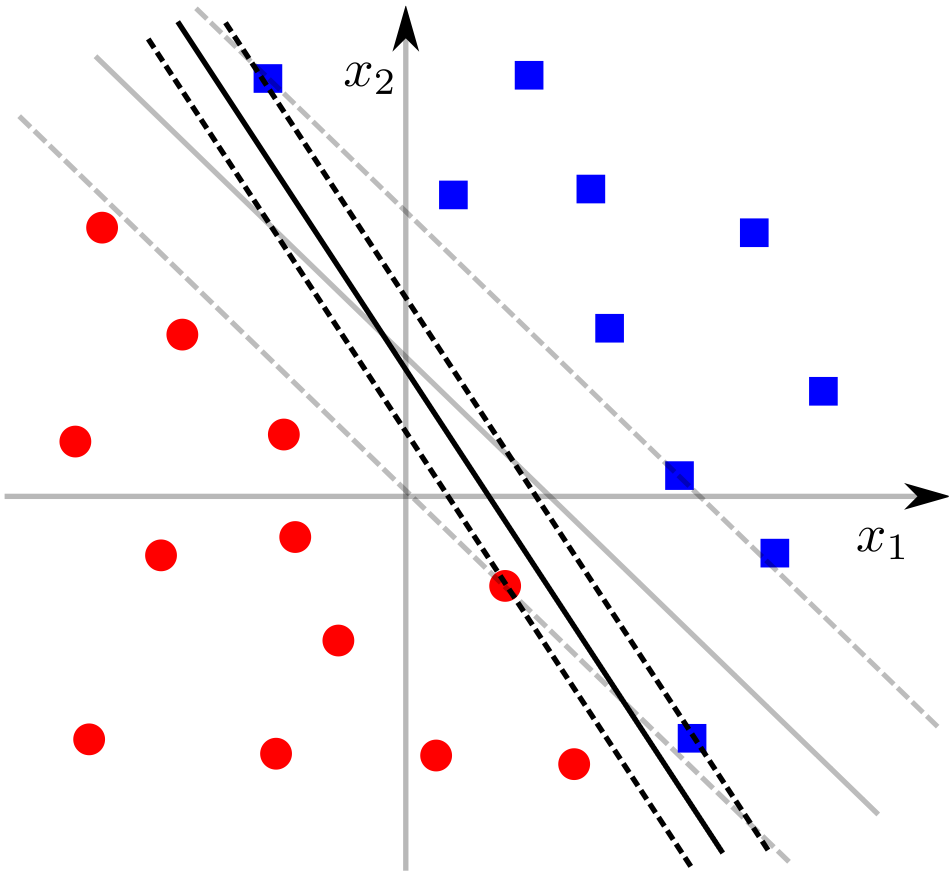
\includegraphics[width=0.7\linewidth]{SoftMarginSVM}
\end{center}
In this situation, the margin become really small just because of the blue sample at the bottom, but such sample could be mislabeled and induce to error. Moreover we should remember that we are not doing optimization, but we are actually still learning, hence probably that point should not be even considered. \newline
There needs to be a trade-off between fitting the training set and generalization, that is fitting on the training data and size of the margin. 
%
%
%
\section{Soft Margin SVM}
The idea is that if even there is a sample which is wrongly labeled in the training phase, we don't really care and prefer a larger margin. 
In hard margin SVM we have:
\[
  \min\limits_{\vect{w},w_0} \frac{\vert\vert \vect{w}\vert\vert^2}{2} s.t. y_i(\vect{w}^T\vect{x}_i +w_0)\geq 1 \forall (\vect{x}_i,y_i)\in\mathcal{D}
\]
To talk about soft margin SVM we need to introduce \textbf{slack variables}.
\begin{definition}[Slack Variable]
  A slack variable $\xi_i$ represents the penalty to pay for example $\vect{x}_i$ not satisfying the margin constraint. 
\end{definition}
The slack variable needs to be non negative, and if it's zero the soft margin becomes hard margin. 
\begin{equation}
  \min\limits_{\vect{w}\in\mathcal{X}, w_0\in\mathbb{R},\xi\in\mathbb{R}^m} \frac{\vert\vert \vect{w}\vert\vert^2}{2}+C\Sum_{i=1}^m\xi_i\quad s.t.\quad 
  \begin{cases}
    y_i(\vect{w}^T\vect{x}_i +w_0)\geq 1 -\xi_i,\quad i=1,\hdots, m\\
    \xi_i\geq 0,\quad i=1,\hdots, m
  \end{cases}
  \label{eq:SoftMargin}
\end{equation}
Where $C\geq0$ is a regularization parameter that trades-off data fitting and the size of the margin, and it's an hyper-parameter. \newline
Notice that if the slack becomes too high, above 1, then we could even have a wrong prediction since the margin becomes smaller than 0. While if the slack variable is $0\leq \xi_i\leq1$, then the margin is soft and its size it's actually $1-\xi_i$. \newline
Soft margin is something that used when we know that the problem is linearly separable but there are some outlayers, which could be simply mislabeled. If the problem is truly non-linearly separable, then we'll see techniques to deal with these problems.
%
%
\subsection{Regularization Theory}
This idea of combining margin ans slack variable is the instance of a more general idea of regularized error minimization and there is a theory, regularization theory, that formalizes this aspect. \newline
The idea is that we have a general loss function $l$:
\[\min\limits_{\vect{w}\in\mathcal{X}, w_0\in\mathbb{R},\xi\in\mathbb{R}^m} \frac{\vert\vert \vect{w}\vert\vert^2}{2}+C\Sum_{i=1}^ml(y_i,f(\vect{x}_i))\]
In this we have two components: the loss term accounts for error minimization, while the margin maximization (minimization of the inverse) accounts for the regularization, i.e., solutions with larger margin are preferred. \newline
Regularization is a standard approach to prevent overfitting. 
%
%
\subsection{Hinge Loss}
The loss function basically is what is measured by the slack variables. The value of the slack is given by the hinge loss: 
\begin{equation}
  l(y_i, f(\vect{x}_i))=\vert1-y_if(\vect{x}_i)\vert_+=\vert1-y_i(\vect{w}^T\vect{x}_i+w_0)\vert_+
  \label{eq:HingeLoss}
\end{equation}
\begin{figure}
  \centering
  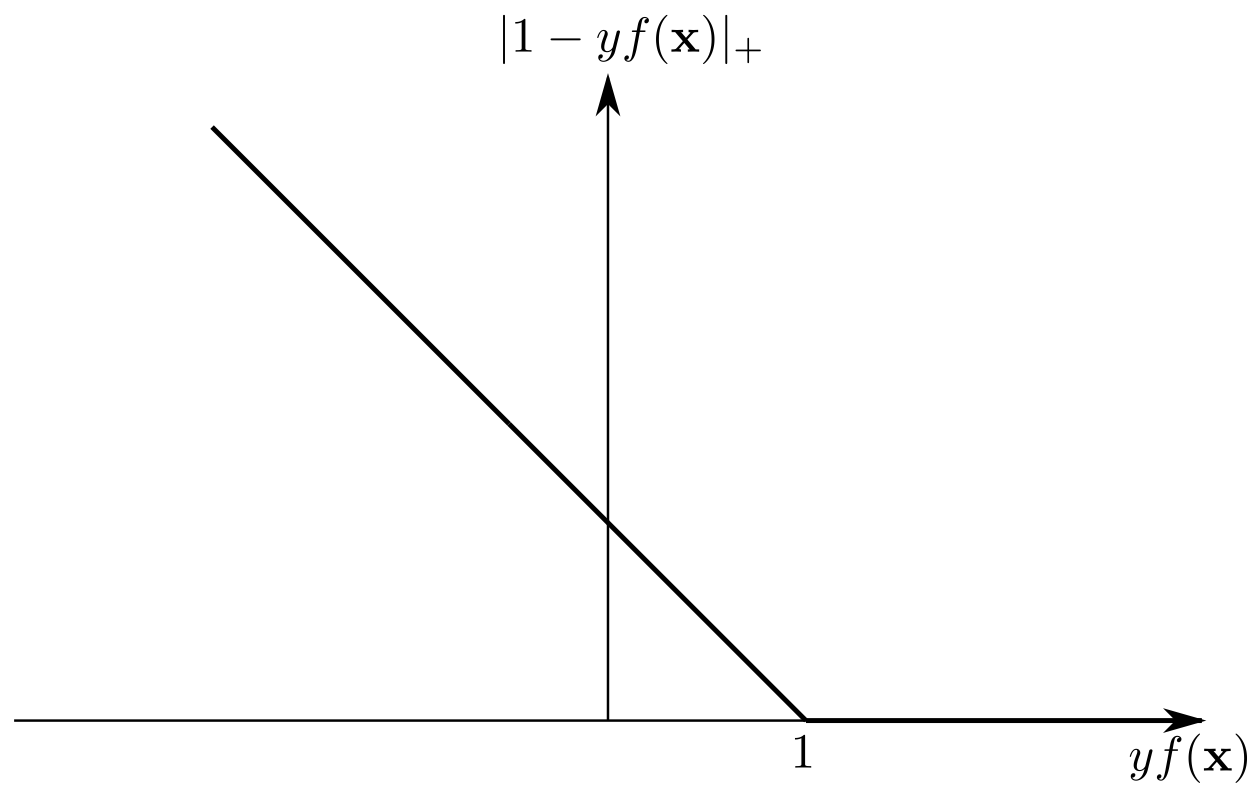
\includegraphics[width=0.7\linewidth]{HingeLoss}
  \caption{The hinge loss function.}
  \label{fig:hingeLoss}
\end{figure}
This is a function of the confidence in the prediction of a correct label. \newline
Since it is computed as the module of 1 minus the confidence, if the module is negative, then the confidence is greater than 1 so we recover the hard margin. \newline
Mind that the notation $\vert f(x)\vert_+$ means that if $f(x)$ is smaller than 0, the value is not $-f(x)$ but $0$, that is $\vert -1\vert_+\neq 1$, but $\vert-1\vert_+=0$. \newline
The nice thing is that it is responsible for bringing the support vectors down to a small number since we are basically removing the hard margin.
%
%
\subsection{Langrangian}
Now we want to find the dual formulation for the soft margin equation (Equation~\ref{eq:SoftMargin}. First thing let's write the Langrangian as done before:
\[
  \mathcal{L}(\vect{w},w_0,\vect{\alpha},\vect{\beta},\vect{\xi})=\frac{\vert\vert \vect{w}\vert\vert^2}{2}+C\Sum_{i=1}^m\xi_i-\Sum_{i=1}^m\alpha_i(y_i(\vect{w}^T\vect{x}_i+w_0)-1-\xi_i)-\Sum_{i=1}^m\beta_i\xi_i 
\]
Where $\alpha_i\geq0$ and $\beta_i\geq0$. \newline
We shall then derive with respect to the primal variables $\vect{w}, w_0, \xi_i$:
\[\frac{\partial}{\partial{w_0}}\mathcal{L}=0\Rightarrow\Sum_{i=1}^m\alpha_iy_i=0\]
\[\frac{\partial}{\partial{\vect{w}}}\mathcal{L}=0\Rightarrow \vect{w}=\Sum_{i=1}^m\alpha_iy_i\vect{x}_i\]
\[\frac{\partial}{\partial{\xi_i}}\mathcal{L}=0\Rightarrow C-\alpha_i-\beta_i=0\]
We can now substitute this value in the Langrangian to obtain the dual formulation:
\[
  \textcolor{red}{\frac{\vert\vert \vect{w}\vert\vert^2}{2}}+
  \textcolor{green}{C\Sum_{i=1}^m\xi_i}-
  \textcolor{blue}{\Sum_{i=1}^m\alpha_i(y_i(\vect{w}^T\vect{x}_i+w_0)-1-\xi_i)}-
  \textcolor{magenta}{\Sum_{i=1}^m\beta_i\xi_i=}
\]
\[
  \textcolor{red}{\frac{1}{2}\vert\vert\vect{w}\vert\vert^2}+
  \textcolor{green}{\Sum_{i=1}^mC\xi_i}-
  \textcolor{blue}{\left(\Sum_{i=1}^m\alpha_iy_i\vect{w}^T\vect{x}_i+\Sum_{i=1}^m\alpha_iy_iw_0-\Sum_{i=1}^m\alpha_i+\Sum_{i=1}^m\alpha_i\xi_i \right)}-
  \textcolor{magenta}{\Sum_{i=1}^m(C-\alpha_i)\xi_i}
\]
We can rewrite $\Sum_{i=1}^m\alpha_iy_i\vect{w}^T\vect{x}_i=\vect{w}^T\Sum_{i=1}^m\alpha_iy_i\vect{x}_i=\vect{w}^T\vect{w}=\vert\vert\vect{w}\vert\vert^2$. 
\[
  \textcolor{red}{\frac{1}{2}\vert\vert\vect{w}\vert\vert^2}+
  \textcolor{green}{\cancel{\Sum_{i=1}^mC\xi_i}}+
  \textcolor{blue}{\Bigg(-\vert\vert\vect{w}\vert\vert^2-w_0}
  \underbrace{\cancel{\textcolor{blue}{\Sum_{i=1}^m\alpha_iy_i}} \rule[-12pt]{0pt}{5pt}}_{\mbox{$=0$}}
  \textcolor{blue}{+\Sum_{i=1}^m\alpha_i-\cancel{\Sum_{i=1}^m\alpha_i\xi_i \Bigg)}}+
  \textcolor{magenta}{\left(-\cancel{\Sum_{i=1}^mC\xi_i}+\cancel{\Sum_{i=1}^m\alpha_i\xi_i}\right)}
\]
Simplifying we obtain:
\[\Sum_{i=1}^m\alpha_i-\frac{1}{2}\vert\vert\vect{w}\vert\vert^2=\Sum_{i=1}^m-\frac{1}{2}\vect{w}^T\vect{w}=\Sum_{i=1}^m\alpha_i-\frac{1}{2}\Sum_{i=1,j=1}^m\alpha_i\alpha_jy_iy_j\vect{x}_i^T\vect{x}_j=\mathcal{L}(\alpha)\]
The dual formulation then require the maximization over $\vect{\alpha}$:
\begin{equation}
  \max\limits_{\vect{\alpha}\in\mathbb{R}^m}\Sum_{i=1}^m\alpha_i-\frac{1}{2}\Sum_{i,j=1}^m\alpha_i\alpha_jy_iy_j\vect{x}_i^T\vect{x}_j\quad s.t.\quad 
\begin{cases}
  0\leq \alpha_i\leq C, i=1,\hdots, m\\
  \Sum_{i=1}^m\alpha_iy_i=0
\end{cases}
\end{equation}
The first constraint for $\alpha_i$ comes from $C-\alpha_i-\beta_i=0$ and the fact that both $\alpha_i$ and $\beta_i$ needs to be greater or equal than 0. \newline
At the saddle point it holds that:
\[
\begin{cases}
  \alpha_i(y-I(\vect{w}^T\vect{x}_i+w_0)-1+\xi_i)=0\\
  \beta_i\xi_i=0
\end{cases}
\forall i
\]
We can distinguish 3 cases:
\begin{itemize}
  \item $\alpha=0$, then the sample it's not a support vector.
  \item $\alpha<C\wedge\alpha\neq0$, then $\beta>0$ and to zero $\beta_i\xi_i$ we need to have $\xi_i=0$. This is the cases for the points that are actually on the confidence one hyperplane. Such points are called \textbf{unbound support vectors}.
  \item $\alpha=C$, then $\xi_i>0$ and the support vectors are margin errors. Such support vector are said \textbf{bound support vectors}.
\end{itemize}
\begin{center}
  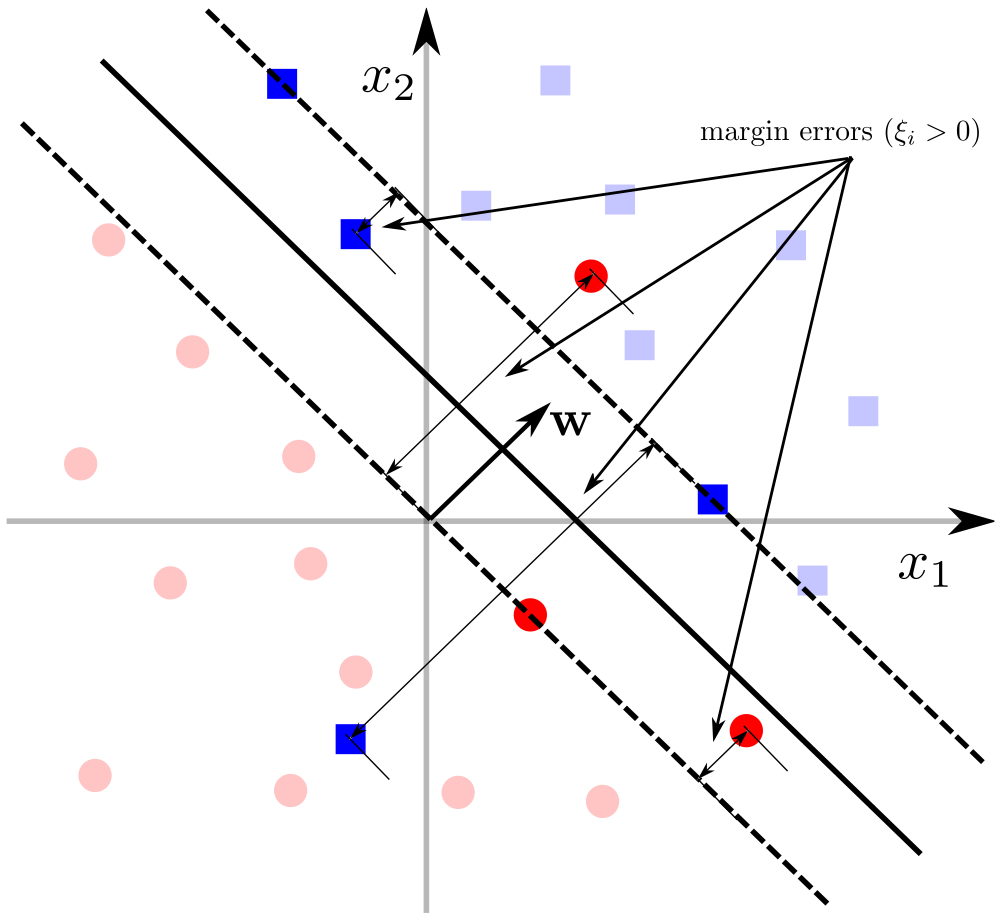
\includegraphics[width=0.7\linewidth]{BoundAndUnboundSV}
\end{center}
%
%
%
\section{Large Scale SVM Learning}
There is no $w_0$ because in large scale the bias is almost irrelevant. \newline
We could plug the hinge loss function inside the minimization procedure and obtain:
\[\min\limits_{\vect{w}\in\mathcal{X}}\frac{\lambda}{2}\vert\vert\vect{w}\vert\vert^2+\frac{1}{m}\Sum_{i=1}^m\vert 1-y_i\langle \vect{w},\vect{x}_i\rangle\vert_+\]
The angular brackets represent an inner product, e.g., scalar product. \newline
Notice that we divide by the number of examples. \newline
Suppose we want to do a full stochastic learning, that is gradient on a single example, then we can write the error function for one example:
\[E(\vect{w};(\vect{x}_i,y_i))=\frac{\lambda}{2}\vert\vert\vect{w}\vert\vert^2+\vert1-y_i\langle\vect{w},\vect{x}_i\rangle\vert_+\]
Which is basically the hinge loss of one example plus the regularization part for the margin. \newline
Since it's a hinge loss, we cannot even compute the gradient, this is pretty noticeable from Figure~\ref{fig:hingeLoss} where we can clearly see that there is a point of discontinuity, we are going to use the subgradient, that is we take only a portion of the function, that is the linear decreasing one:
\[\nabla_{\vect{w}}E(\vect{w};(\vect{x}_i,y_i))=\lambda\vect{w}-\mathbf{1}[y_i\langle\vect{w},\vect{x}_i\rangle<1]y_i\vect{x}_i\]
The indicator function is such that:
\[\mathbf{1}[y_i\langle\vect{w},\vect{x}_i\rangle<1]=
  \begin{cases}
    1\qquad\text{if }y_i\langle\vect{w},\vect{x}_i\rangle<1\\
    0\qquad\text{otherwise}
  \end{cases}
\]
The subgradient of a function $f$ at a point $\vect{x}_0$ is any vector $\vect{v}$ such that for any $\vect{x}$:
\[f(\vect{x})-f(\vect{x}_0)=\geq\vect{v}^T(\vect{x}-\vect{x}_0)\]
Basically the subgradient is the coefficient for any line that goes through $\vect{x}_0$ and is below the function. In the hinge loss, considering $x_0=1$, the subgradient is any value that is less than the initial slope and that is still greater than 0. 
We can compute the subgradient stochastically as follows:
\begin{enumerate}
  \item Initialize $\vect{w}_1=0$
  \item For $t=1$ to $T$:
    \begin{enumerate}
      \item Randomly choose $(\vect{x}_{i_t}, y_{i_t})$ from $\mathcal{D}$:
      \item Set $\eta_t=\frac{1}{\lambda t}$
      \item Update $\vect{w}$:
        \[\vect{w}_{t+1}=\vect{w}_t-\eta_t\lambda_{\vect{w}}E(\vect{w};(\vect{x}_{i_t},y_{i_t}))\]
    \end{enumerate}
  \item Return $\vect{w}_{T+1}$
\end{enumerate}
The choice of the learning rate allows to bound the runtime for an $\epsilon$ accurate solution $O(\myfrac{d}{\lambda\epsilon}$ with $d$ maximum number of non-zero features in an example. 
This algorithm is called Pegasus. 

\section{Non Linear Support Vector Machine}
We saw that hard margin SVM can address linearly separable problems and that soft margin SVM can solve linearly separable problem with outliers. None of them though works for non-linearly separable problem for which we need a higher expressive power. \newline
The goal is to find a way to solve non-linearly separable problems yet maintaining the advantages of linear separators. One possible way of achieving this is by mapping input examples in a higher dimensional feature space and then perform linear classification. \newline
We define a feature map $\phi$ such that each example is mapped into a larger feature dimensional space. 
\[\phi:\mathcal{X}\rightarrow \mathcal{H}\]
Each example $\vect{x}$ gets replaced by its feature mapping $\phi(x)$. \newline
The idea is that $\phi$ should give more expressive power of the representation, e.g., introducing features which are the combinations of input features, and in the new mapped space, examples should be linearly separable. \newline
We can distinguish two types of mapping:
\begin{itemize}
  \item \textbf{Homogeneous}: we map features to all possible conjunctions of features of a certain degree $d$:
    \[\phi 
      \begin{pmatrix}
        x_1\\x_2
      \end{pmatrix}=
      \begin{pmatrix}
        x_1^2\\
        x_1x_2\\
        x_2^2
      \end{pmatrix}
    \]
  \item \textbf{Inhomogeneous}: we map features to all possible conjunctions of features up to a certain degree $d$:
    \[\phi 
      \begin{pmatrix}
        x_1\\x_2
      \end{pmatrix}=
      \begin{pmatrix}
        x_1\\
        x_2\\
        x_1^2\\
        x_1x_2\\
        x_2^2
      \end{pmatrix}
    \]
\end{itemize}
Let's consider the case in which we have the following examples:
\begin{center}
  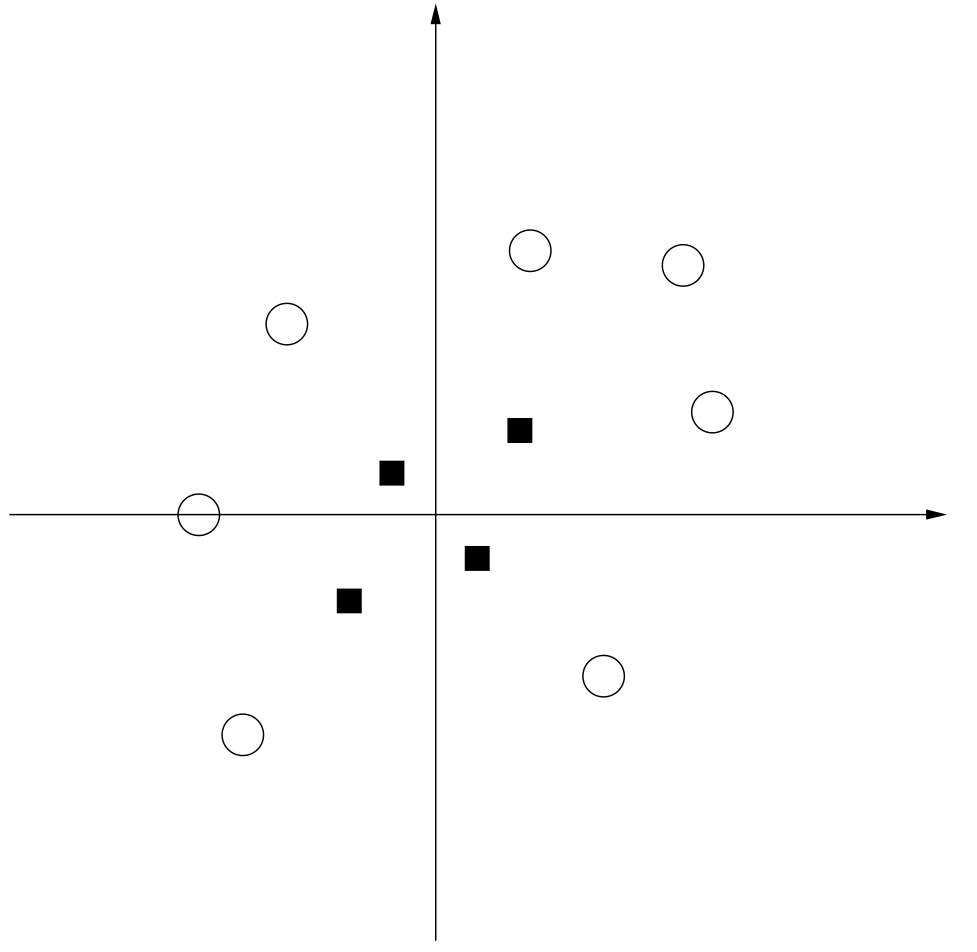
\includegraphics[width=0.5\linewidth]{NLSVMExample1_1}
\end{center}
Clearly they are not linearly separable, but when we map them into a higher dimensional space, we see that there actually is an hyperplane that separates them:
\begin{center}
  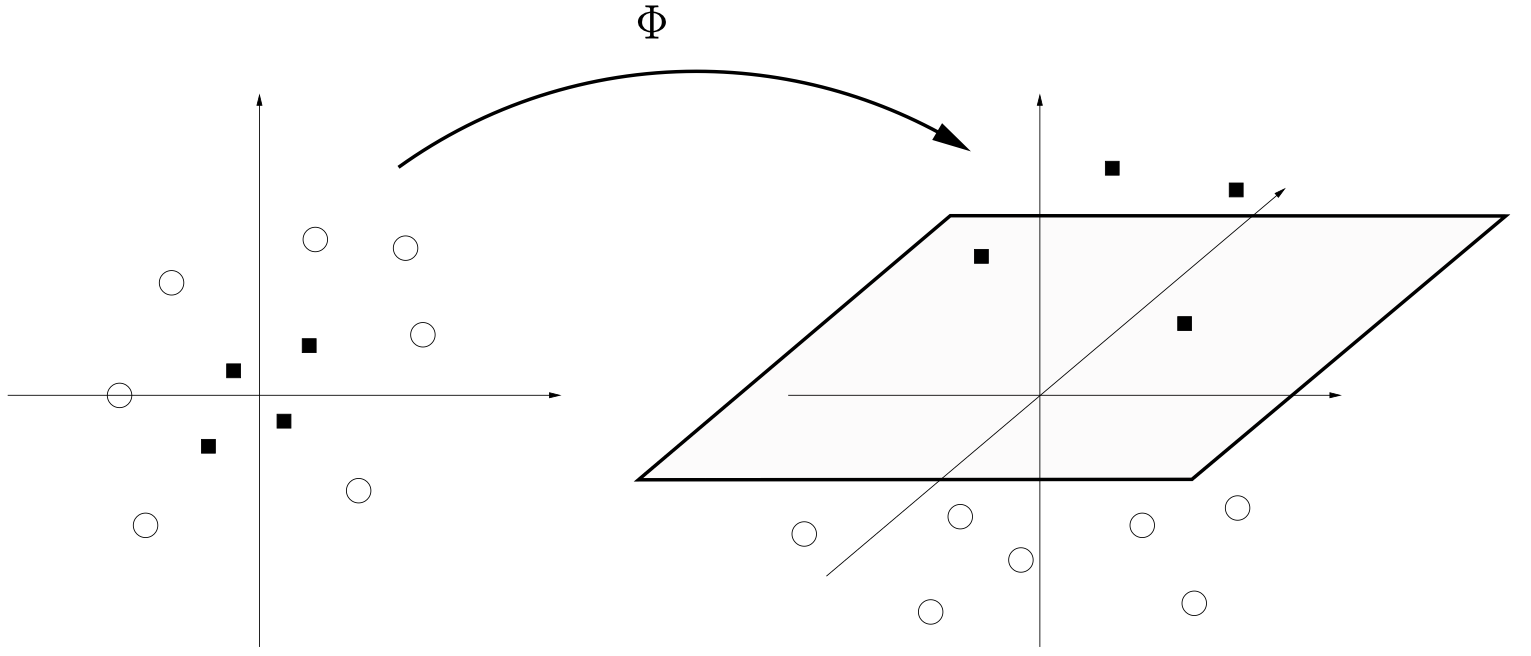
\includegraphics[width=0.7\linewidth]{NLSVMExample1_2}
\end{center}
What we actually need to find now is a function $f$ such that it can map the separating hyperplane back to the orginal feature space $\mathcal{X}$.
\begin{center}
  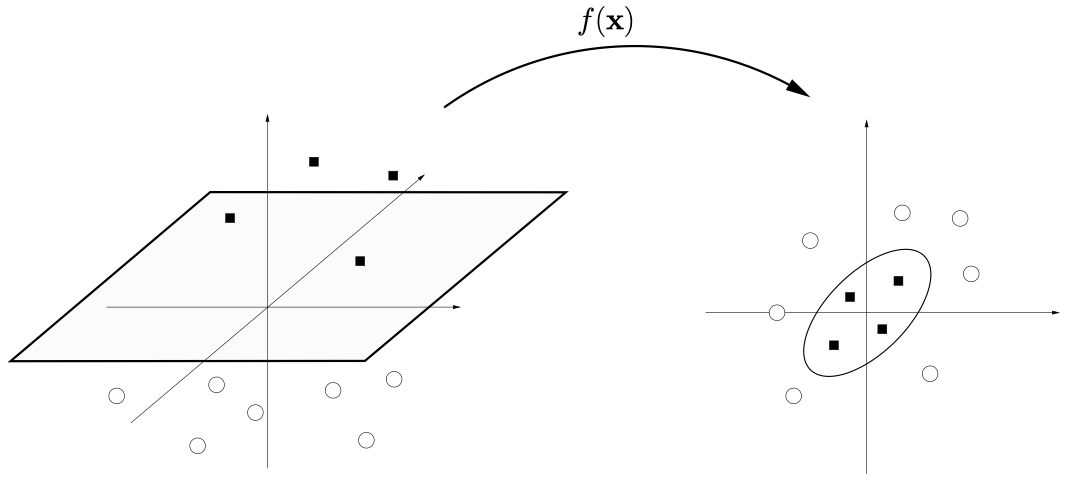
\includegraphics[width=0.7\linewidth]{NLSVMExample1_3}
\end{center}
But this is actually straight forward: a linear separation in feature space corresponds to a non-linear separation in input space just by replacing $\vect{x}$ with $\phi(\vect{x})$:
\[f(\vect{x})=\vect{w}^T\phi(\vect{x})+w_0\]
where $\vect{w}$ is in the mapping space. \newline
For example, if we'd applied a homogeneous mapping function of degree 2, we'd have:
\[f
\begin{pmatrix}
  x_1\\
  x_2
\end{pmatrix}=
\sign(w_1x_1^2+w_2x_1x_2+w_3x_2^2+w_0)
\]
Note that this is called \textbf{polynomial mapping}, that is we take the vector and apply all possible combinations of multiplication between features. This is really simple yet useful. \newline
In some cases applying a higher dimensional space is not possible since the initial space is already large, or even infinite. We'll see how to deal with these cases. 
%
%
\subsection{Support Vector Regression}
To go into regression we would like to have an extension of the hinge loss, and we can do this by adding a tolerance region for the examples:
\begin{equation}
  l(f(\vect{x})y)=\vert y-f(\vect{x})\vert_\epsilon=
  \begin{cases}
    \begin{array}{ll}
      0&\text{if }\vert y-f(\vect{x})\vert\leq \epsilon\\
      \vert y-f(\vect{x})\vert-\epsilon&\text{otherwise}
    \end{array}
  \end{cases}
  \label{eq:InsensitiveLoss}
\end{equation}
This new loss function is called $\epsilon$\textbf{-insensitive loss} and it allow to tolerate small ($\epsilon$) deviations from the true value without having any penalty. What this does, is to define an $\epsilon$-tube of insensitiveness around the true values. This also allows to trade off function complexity with data fitting by playing with $\epsilon$. 
The optimization problem is the following:
\begin{equation}
  \min\limits_{\vect{w}\in\mathcal{X},w_0\in\mathbb{R},\vect{\xi},\vect{\xi}^*\in\mathbb{R}^m}\frac{1}{2}\vert\vert\vect{w}\vert\vert^2+C\Sum_{i=1}^m(\xi_i+\xi_i^*)\quad s.t.\quad 
  \begin{cases}
    \vect{w}^T\phi(\vect{x}_i)+w_0-y_i\leq \epsilon+\xi_i\\
    y_i-(\vect{w}^T\phi(\vect{x}_i)+w_0)\leq \epsilon+\xi_i^*\\
    \xi_i\xi_i^*\geq 0
  \end{cases}
  \label{eq:SVMRegression}
\end{equation}
The first two constraints actually works by constraining the upper and lower side of the tube for each example. The last add slack variables $\xi_i,\xi_i^*$ penalizing predictions out of the $\epsilon$-insensitive tube. \newline
Basically we start from wanting to minimize the normal weight, which is subject to the constraints about the insensitiveness, that is we want the prediction to be inside a certain margin $\epsilon$:
\[\min\limits_{\vect{w}\in\mathcal{X}}\frac{\vert\vert\vect{w}\vert\vert^2}{2}\quad s.t.\quad 
\begin{cases}
  y_i-f(\vect{x}_i)\leq \epsilon\\
  f(\vect{x}_i)-y_i\leq \epsilon
\end{cases},\quad\forall i
\]
This allows us to assume that all training instances are within $\epsilon$ from the real value, hence the prediction is out of at mose $\epsilon$. \newline
As in classification we can relax the constraints by adding slack variables. Since there are two constraints, we need to slack variables:
\[\min\limits_{\vect{w}\in\mathcal{X}}\frac{\vert\vert\vect{w}\vert\vert^2}{2}+C\Sum_{i=1}^m(\xi_i+\xi^*_i)\quad s.t.\quad 
\begin{cases}
  y_i-f(\vect{x}_i)\leq \epsilon+\xi^*_i\\
  f(\vect{x}_i)-y_i\leq \epsilon+\xi_i\\
  \xi_i,\xi_i^*\geq0 
\end{cases}
\]
By rewriting $f(x)=\vect{w}^T\phi(\vect{x}_i)+w_0$ we obtain again Equation~\ref{eq:SVMRegression}. \newline
As done with classification, let's now use Karush-Kuhn-Tucker approach, include the slack variables and obtain the Langrangian by using Langrangia multipiers ($\alpha_i,\alpha_i^*,\beta_i,\beta_i^*\geq 0)$:\[
  \mathcal{L}=\frac{1}{2}\vert\vert\vect{w}\vert\vert^2+C\Sum_{i=1}^m(\xi_i+\xi_i^*)-\Sum_{i=1}^m(\beta_i\xi_i+\beta_i^*\xi_i^*)+\]\[
  -\Sum_{i=1}^m\alpha_i(\epsilon+\xi_i+y_i-\vect{w}^T\phi(\vect{x}_i)-w_0)-\Sum_{i=1}^m\alpha_i^*(\epsilon+\xi_i^*-y_i+\vect{w}^T\phi(\vect{x}_i)+w_0)
\]
We shall then minimize the primal variables:
\[\frac{\partial\mathcal{L}}{\partial\vect{w}}=\vect{w}-\Sum_{i=1}^m(\alpha_i^*-\alpha_i)\phi(\vect{x}_i)=0\rightarrow\vect{w}=\Sum_{i=1}^m(\alpha_i^*-\alpha_i)\phi(\vect{x}_i)\]
\[\frac{\partial\mathcal{L}}{\partial w_0}=\Sum_{i=1}^m(\alpha_i-\alpha_i^*)=0\]
\[\frac{\partial\mathcal{L}}{\partial\xi_i}=C-\alpha_i-\beta_i=0\rightarrow\alpha_i\in[0,C]\]
\[\frac{\partial\mathcal{L}}{\partial\xi_i^*}=C-\alpha_i^*-\beta_i^*=0\rightarrow\alpha_i^*\in[0,C]\]
Then we work on the Langrangian to find the dual formulation:
\[
  \begin{array}{c}
    \mathcal{L}=\frac{1}{2}\vert\vert\vect{w}\vert\vert^2+C\Sum_{i=1}^m(\xi_i+\xi_i^*)-\Sum_{i=1}^m(\beta_i\xi_i+\beta_i^*\xi_i^*)+\\
    -\Sum_{i=1}^m\alpha_i(\epsilon+\xi_i+y_i-\vect{w}^T\phi(\vect{x}_i)-w_0)-\Sum_{i=1}^m\alpha_i^*(\epsilon+\xi_i^*-y_i+\vect{w}^T\phi(\vect{x}_i)+w_0)=
  \end{array}
\]
\[
  \begin{array}{c}
    =\frac{1}{2}\vect{w}^T\vect{w}+\Sum_{i=1}^mC\xi_i+\Sum_{i=1}^mC\xi_i^*-\Sum_{i=1}^m\beta_i\xi_i-\Sum_{i=1}^m\beta_i^*\xi_i^*+\\
    -\left(\Sum_{i=1}^m\alpha_i\epsilon +\Sum_{i=1}^m\alpha_i\xi_i+\Sum_{i=1}^m\alpha_iy_i-\Sum_{i=1}^m\alpha_i\vect{w}^T\phi(\vect{x}_i)-\Sum_{i=1}^m\alpha_iw_0\right)+\\
    -\left(\Sum_{i=1}^m\alpha_i^*\epsilon +\Sum_{i=1}^m\alpha_i^*\xi_i^*-\Sum_{i=1}^m\alpha_i^*y_i+\Sum_{i=1}^m\alpha_i^*\vect{w}^T\phi(\vect{x}_i)+\Sum_{i=1}^m\alpha_i^*w_0\right)=\\
  \end{array}
\]
\[
  \begin{array}{c}
    =\frac{1}{2}\Sum_{i=1}^m(\alpha_i^*-\alpha_i)\phi(\vect{x}_i)^T\Sum_{i=1}^m(\alpha_i^*-\alpha_i)\phi(\vect{x}_i)+\Sum_{i=1}^mC\xi_i+\Sum_{i=1}^mC\xi_i^*-\Sum_{i=1}^m\beta_i\xi_i-\Sum_{i=1}^m\beta_i^*\xi_i^*+\\
    -\Sum_{i=1}^m\alpha_i\xi_i-\Sum_{i=1}^m\alpha_i^*\xi_i^*+\Sum_{i=1}^m\alpha_iw_0-\Sum_{i=1}^m\alpha_i^*w_0-\Sum_{i=1}^m\alpha_i\epsilon-\Sum_{i=1}^m\alpha_i^*\epsilon -\Sum_{i=1}^m\alpha_iy_i+\Sum_{i=1}^m\alpha_i^*y_i+\\
    +\Sum_{i=1}^m\alpha_i\vect{w}^T\phi(\vect{x}_i)-\Sum_{i=1}^m\alpha_i^*\vect{w}^T\phi(\vect{x}_i)
  \end{array}
\]
\[
  \begin{array}{c}
    =\frac{1}{2}\Sum_{i,j=1}^m(\alpha_i^*-\alpha_i)(\alpha_j^*-\alpha_j)\phi(\vect{x}_i)^T\phi(\vect{x}_j)+\Sum_{i=1}^m\xi_i(
      \underbrace{C-\beta_i-\alpha_i \rule[-12pt]{0pt}{5pt}}_{\mbox{$=0$}})+\Sum_{i=1}^m\xi_i^*(
      \underbrace{C-\beta_i-\alpha_i \rule[-12pt]{0pt}{5pt}}_{\mbox{$=0$}})+\\
    +w_0
      \underbrace{\Sum_{i=1}^m(\alpha_i-\alpha_i^*) \rule[-12pt]{0pt}{5pt}}_{\mbox{$=0$}}-\epsilon\Sum_{i=1}^m(\alpha_i+\alpha_i^*)+\Sum_{i=1}^my_i(\alpha_i^*-\alpha_i)-\vect{w}^T
      \underbrace{\Sum_{i=1}^m\phi(\vect{x}_i)(\alpha_i^*-\alpha_i) \rule[-12pt]{0pt}{5pt}}_{\mbox{$=\vect{w}$}}
  \end{array}
\]
\[
  =\frac{1}{2}\Sum_{i,j=1}^m(\alpha_i^*-\alpha_i)(\alpha_j^*-\alpha_j)\phi(\vect{x}_i)^T\phi(\vect{x}_j)-\epsilon\Sum_{i=1}^m(\alpha_i+\alpha_i^*)+\Sum_{i=1}^my_i(\alpha_i^*-\alpha_i)-\vect{w}^T\vect{w}=
\]
\[
  \begin{array}{c}
    =\frac{1}{2}\Sum_{i,j=1}^m(\alpha_i^*-\alpha_i)(\alpha_j^*-\alpha_j)\phi(\vect{x}_i)^T\phi(\vect{x}_j)-\Sum_{i,j=1}^m(\alpha_i^*-\alpha_i)(\alpha_j^*-\alpha_j)\phi(\vect{x}_i)^T\phi(\vect{x}_j)\\
    -\epsilon\Sum_{i=1}^m(\alpha_i+\alpha_i^*)+\Sum_{i=1}^my_i(\alpha_i^*-\alpha_i)=
  \end{array}
\]
\[
  =-\frac{1}{2}\Sum_{i,j=1}^m(\alpha_i^*-\alpha_i)(\alpha_j^*-\alpha_j)\phi(\vect{x}_i)^T\phi(\vect{x}_j)-\epsilon\Sum_{i=1}^m(\alpha_i+\alpha_i^*)+\Sum_{i=1}^my_i(\alpha_i^*-\alpha_i)
\]
Obtaining the dual formulation:
\[\max\limits_{\vect{\alpha}\in\mathbb{R}^m}-\frac{1}{2}\Sum_{i,j=1}^m(\alpha_i^*-\alpha_i)(\alpha_j^*-\alpha_j)\phi(\vect{x}_i^T\phi(\vect{x}_j)-\epsilon\Sum_{i=1}^m(\alpha_i^*+\alpha_i)+\Sum_{i=1}^my_i(\alpha_i^*-\alpha_i)\quad s.t.\quad 
  \begin{cases}
    \Sum_{i=1}^m(\alpha_i-\alpha_i^*)=0\\
    \alpha_i,\alpha_i^*\in[0,C], \quad \forall i \in[1,m]
  \end{cases}
\]
By substituting $\vect{w}$ with the value we obtained before while derivating, we can rewrite the regression function as:
\[f(\vect{x})=\vect{w}^T\phi(\vect{x}+w_0=\Sum_{i=1}^m(\alpha_i-\alpha_i^*)\phi(\vect{x})+w_0\]
At the saddle point it holds that for all $i$:
\[
  \begin{cases}
    \alpha_i(\epsilon+\xi_i+y_i-\vect{w}^T\phi(\vect{x}_i)-w_0)=0\\
    \alpha_i^*(\epsilon+\xi_i^*+y_i-\vect{w}^T\phi(\vect{x}_i)-w_0)=0\\
    \beta_i\xi_i=0
    \beta_i^*\xi_i^*=0
  \end{cases}
\]
Combining this with the constraints:
\[
\begin{cases}
  C-\alpha_i-\beta_i=0\\
  C-\alpha_i^*-\beta_i^*=0\\
  \alpha_i\geq 0\\
  \alpha_i^*\geq 0\\
  \beta_i\geq 0
  \beta_i^*\geq 0
\end{cases}
\]
we get:
\[\alpha_i=C~\text{ if }~\xi_i>0,\qquad\alpha_i^*=C~\text{ if }~\xi_i^*>0\]
So we can distinguish some cases:
\begin{itemize}
  \item All patterns within the $\epsilon$-tube, for which $\vert f(\vect{x}_i)-y_i\vert<\epsilon$, have $\alpha_i,\alpha_i^*=0$ and thus don't contribute to the estimated function $f$.
  \item Pattern for which either $0<\alpha_i<C$ or $0<\alpha_i^*<C$ are on the border of the $\epsilon$-tube, that is $\vert f(\vect{x}_i)-y_i\vert=\epsilon$. They are the unbound support vectors.
  \item The remaining training patterns are margin errors (either $\xi_i>0$ or $\xi_i^*>0$) and reside out of the $\epsilon$-insensitive region. They are bound support vectors, with corresponding $\alpha_i=C$ or $\alpha_i^*=C$.
\end{itemize}
\begin{center}
  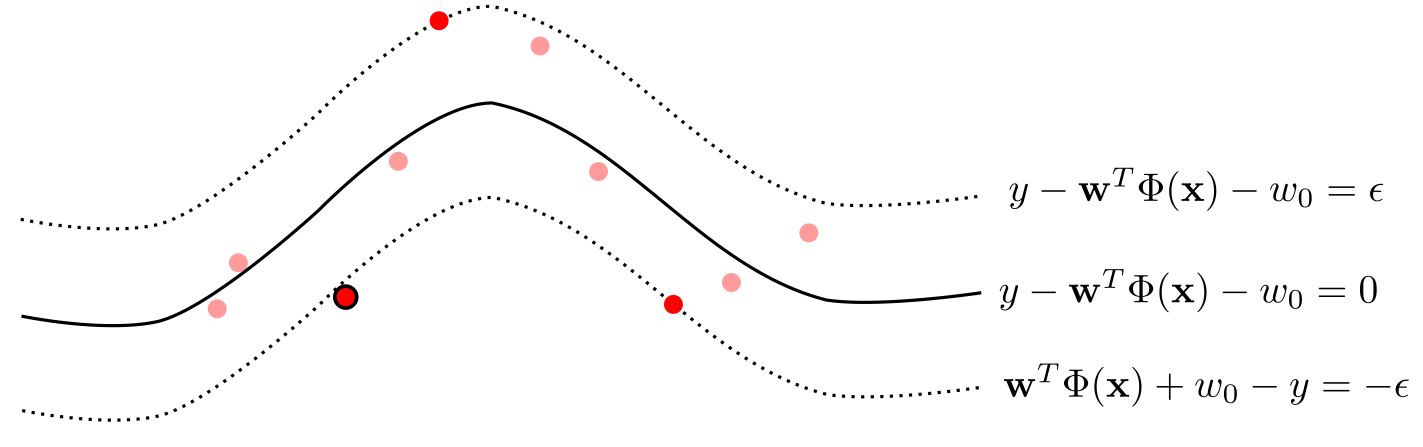
\includegraphics[width=0.7\linewidth]{NLSVMRegression1}
\end{center}
In the following figure it's possible to see how the $\epsilon$-insensitive region influences also the support vectors.
\begin{center}
  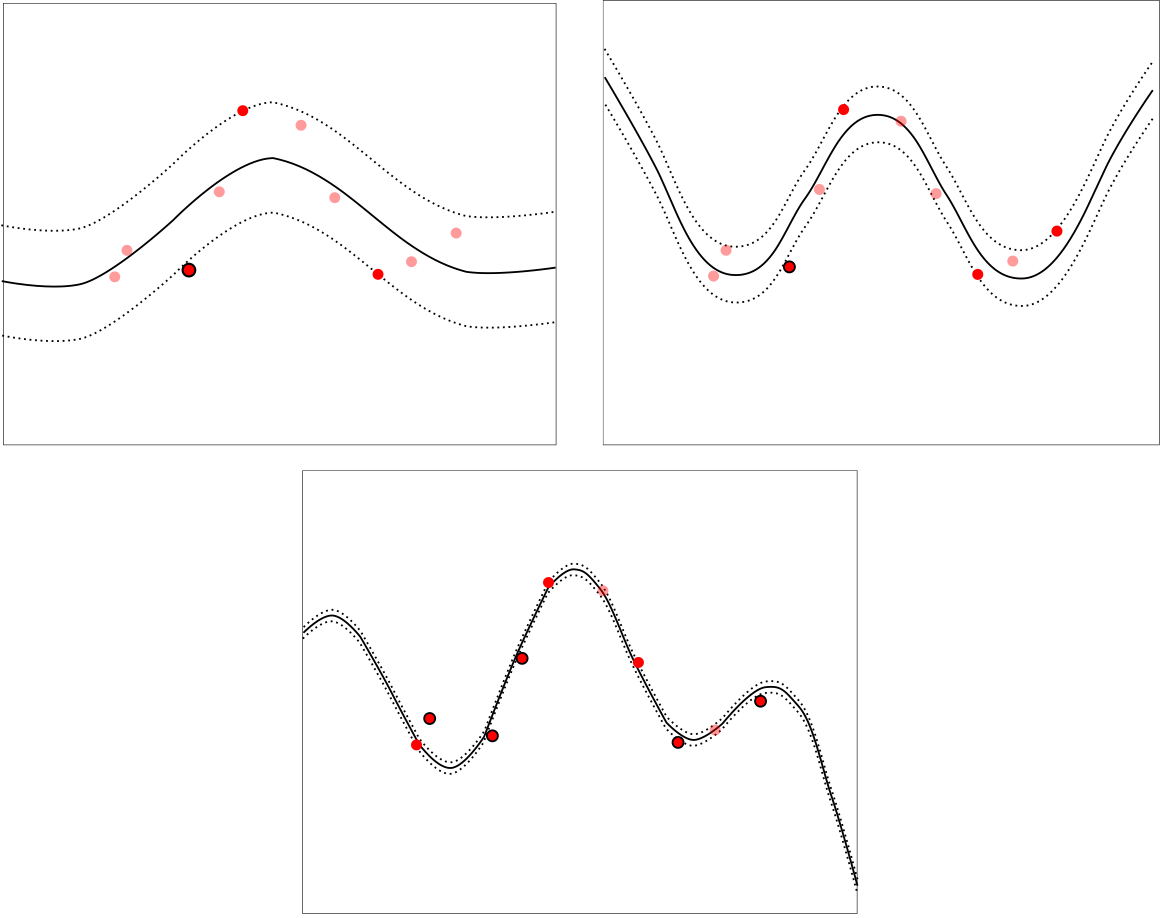
\includegraphics[width=0.7\linewidth]{NLSVMRegression2}
\end{center}


%\data{20/11/2020}

